\chapter{Ordinary Differential Equations and Dynamical Systems}
\label{chap:04-ordinary-differential-equations}
\chapteropeningart{Laws of change}{A differential equation does not merely describe a state; it specifies how one state produces the next.}

\begin{roadmapbox}
Physical laws as evolution equations $\longrightarrow$ first-order initial-value problems $\longrightarrow$ second-order motion $\longrightarrow$ coupled systems $\longrightarrow$ phase space, equilibrium, and stability $\longrightarrow$ nonlinear dynamics and numerical evolution.
\end{roadmapbox}

\learningobjectives
\begin{itemize}
\item translate a verbal law of change into an ordinary differential equation;
\item distinguish general solutions, particular solutions, and initial-value problems;
\item solve separable and first-order linear equations and interpret their characteristic time scales;
\item derive and classify free, damped, and driven oscillator equations;
\item rewrite higher-order equations as first-order systems and analyze them using matrices;
\item read direction fields and phase portraits as geometric representations of dynamics;
\item classify equilibria by linearization and connect stability to physical behavior.
\end{itemize}

\newpage
\section{Differential Equations as Laws of Change}
\label{sec:ch4-laws-of-change}

A function records how one quantity depends on another. A differential equation goes further: it constrains the rate at which that function may change. In physics this distinction is fundamental. A position $x(t)$ is a description of motion; Newton's law is a rule that selects the physically allowed motions from all imaginable curves.

\begin{definitionbox}[Ordinary differential equation]
An \emph{ordinary differential equation} (ODE) is a relation involving an unknown function of one independent variable and one or more of its derivatives. Its order is the order of the highest derivative that appears.
\end{definitionbox}

Examples include
\begin{align}
\frac{dN}{dt}&=-\lambda N, &\text{radioactive decay},\\
C\frac{dV}{dt}+\frac{1}{R}V&=\frac{1}{R}V_{\mathrm{in}}, &\text{RC circuit},\\
m\frac{d^2x}{dt^2}+kx&=0, &\text{harmonic oscillator}.
\end{align}
The symbols differ, but the logic is the same: the present state and the law determine how the system evolves.

\begin{keyidea}[State plus law plus initial data]
A deterministic initial-value problem has three ingredients:
\[
\text{state variables}+\text{evolution law}+\text{initial data}.
\]
The differential equation supplies local change; the initial condition selects one trajectory from the family of mathematically possible solutions.
\end{keyidea}

\subsection{General and particular solutions}
For
\[
\frac{dy}{dt}=ay,
\]
separation gives the family
\[
y(t)=Ce^{at}.
\]
The arbitrary constant $C$ represents missing information. If $y(0)=y_0$, then $C=y_0$ and the initial-value problem has the particular solution
\[
\boxed{y(t)=y_0e^{at}}.
\]
Thus integration constants are not algebraic leftovers; they encode the freedom fixed by physical preparation.

\subsection{Existence, uniqueness, and predictability}
An equation may have no solution, one solution, or many solutions through the same initial point. For a first-order equation
\[
\dot y=f(t,y),
\]
continuity of $f$ near $(t_0,y_0)$ supports local existence, while a local Lipschitz condition in $y$ supports uniqueness. The precise theorem will be developed later, but its physical meaning is immediate: uniqueness is the mathematical form of deterministic prediction.

\begin{mistakebox}[A formula is not automatically a law]
Writing $y(t)=t^2$ describes one curve. Writing $\dot y=2t$ specifies a family of curves, and adding $y(0)=0$ selects the particular curve $t^2$. Description, law, and initial condition must not be confused.
\end{mistakebox}

\subsection{Autonomous and nonautonomous equations}
An ODE is \emph{autonomous} when the independent variable does not appear explicitly:
\[
\dot y=f(y).
\]
It is \emph{nonautonomous} when external time dependence appears:
\[
\dot y=f(t,y).
\]
Autonomous equations are naturally represented in phase space because the velocity at a state depends only on that state. Nonautonomous equations often describe externally driven systems.

\begin{historybox}[From geometric motion to differential law]
Newton formulated motion through fluxions and forces; Leibniz supplied the differential notation that made rates of change algebraically portable. Euler systematized differential equations as a distinct subject, while Cauchy placed initial-value problems and local existence on a more rigorous foundation. Their combined legacy is the modern idea that a physical law is an evolution rule posed together with data.
\end{historybox}

\begin{physicalbox}[Connection to physics]
The same architecture recurs throughout the book. Newton's equation evolves position and momentum; Maxwell's equations evolve electromagnetic fields; the Schrödinger equation evolves a quantum state; diffusion equations evolve density; Einstein's equations constrain the geometry of spacetime. The mathematical details change, but the central question remains: given a state now, what states are allowed next?
\end{physicalbox}

\begin{figure}[htbp]
\centering
\begin{tikzpicture}[node distance=1.15cm and 1.45cm, every node/.style={font=\small}]
\node[draw,rounded corners,fill=softblue,minimum width=3.2cm,minimum height=.9cm] (state) {State $\mathbf{x}(t_0)$};
\node[draw,rounded corners,fill=softgreen,right=of state,minimum width=3.2cm,minimum height=.9cm] (law) {Law $\dot{\mathbf{x}}=\mathbf{f}$};
\node[draw,rounded corners,fill=softgold,right=of law,minimum width=3.2cm,minimum height=.9cm] (traj) {Trajectory $\mathbf{x}(t)$};
\draw[->,thick] (state)--(law);
\draw[->,thick] (law)--(traj);
\node[below=of law,draw,rounded corners,fill=softgray,minimum width=4.1cm] (data) {Parameters and initial conditions};
\draw[->,thick] (data)--(law);
\end{tikzpicture}

\caption{The architecture of deterministic evolution: a state, a law, and initial data define a trajectory.}
\label{fig:ch4-evolution-architecture}
\end{figure}

\section{First-Order Differential Equations}
\label{sec:ch4-first-order}

A first-order ODE relates a function to its first derivative. Although simple in form, such equations already model decay, charging, cooling, relaxation, transport, and population growth.

\subsection{Separable equations}
An equation is separable when it can be written
\[
\frac{dy}{dt}=g(t)h(y).
\]
Where $h(y)\neq0$, rearrange and integrate:
\[
\int \frac{dy}{h(y)}=\int g(t)\,dt+C.
\]
The method is justified by the chain rule, not by treating $dy$ and $dt$ as independent numbers.

\begin{workedexample}
A sample contains $N_0$ unstable nuclei and obeys $\dot N=-\lambda N$ with $\lambda>0$. Find $N(t)$ and the half-life.
\begin{solution}
Separate variables:
\[
\frac{dN}{N}=-\lambda\,dt.
\]
Integrating gives $\ln N=-\lambda t+C$, hence
\[
N(t)=N_0e^{-\lambda t}.
\]
The half-life $t_{1/2}$ satisfies $N(t_{1/2})=N_0/2$, so
\[
\boxed{t_{1/2}=\frac{\ln2}{\lambda}}.
\]
\end{solution}
The inverse rate $\tau=1/\lambda$ is the characteristic decay time.
\end{workedexample}

\subsection{First-order linear equations}
The standard form is
\[
\dot y+p(t)y=q(t).
\]
Multiplication by the integrating factor
\[
\mu(t)=\exp\left(\int p(t)\,dt\right)
\]
turns the left side into a product derivative:
\[
\frac{d}{dt}\bigl(\mu y\bigr)=\mu q.
\]
Therefore
\[
\boxed{y(t)=\frac{1}{\mu(t)}\left[C+\int^t\mu(s)q(s)\,ds\right]}.
\]

\begin{workedexample}
A body at temperature $T(t)$ is placed in an environment at constant temperature $T_a$. Newton's cooling law is
\[
\dot T=-k(T-T_a),\qquad k>0.
\]
For $T(0)=T_0$, determine $T(t)$.
\begin{solution}
Set $u=T-T_a$. Then $\dot u=-ku$, so
\[
u(t)=(T_0-T_a)e^{-kt}.
\]
Hence
\[
\boxed{T(t)=T_a+(T_0-T_a)e^{-kt}}.
\]
\end{solution}
The difference from equilibrium decays exponentially; the ambient temperature is a stable fixed point.
\end{workedexample}

\subsection{Equilibria and qualitative behavior}
For an autonomous equation $\dot y=f(y)$, an equilibrium $y_*$ satisfies $f(y_*)=0$. The sign of $f$ on either side determines whether neighboring solutions move toward or away from $y_*$. This one-dimensional phase-line analysis anticipates the stability theory of systems.

For the logistic equation
\[
\dot P=rP\left(1-\frac{P}{K}\right),
\]
the equilibria are $P=0$ and $P=K$. For $r>0$, small positive populations grow away from zero and toward the carrying capacity $K$.

\begin{workedexample}
Solve the logistic initial-value problem $\dot P=rP(1-P/K)$, $P(0)=P_0>0$.
\begin{solution}
Partial fractions give
\[
\frac{1}{P(1-P/K)}=\frac{1}{P}+\frac{1}{K-P}.
\]
Integration yields
\[
\ln\frac{P}{K-P}=rt+C.
\]
Using the initial condition,
\[
\boxed{P(t)=\frac{K}{1+\left(\frac{K-P_0}{P_0}\right)e^{-rt}}}.
\]
\end{solution}
The early-time behavior is approximately exponential, while nonlinear feedback produces saturation.
\end{workedexample}

\subsection{Direction fields}
The differential equation $\dot y=f(t,y)$ assigns a slope to every point in the $(t,y)$ plane. Drawing short line segments of slope $f(t,y)$ produces a direction field. A solution curve is tangent to this field everywhere.

\begin{figure}[htbp]
\centering
\begin{tikzpicture}[x=1.0cm,y=.65cm]
\draw[->] (-3.4,0)--(3.6,0) node[right] {$t$};
\draw[->] (0,-3.4)--(0,3.5) node[above] {$y$};
\foreach \x in {-3,-2.5,...,3}{\foreach \y in {-3,-2.5,...,3}{\pgfmathsetmacro{\ang}{atan(-\y)}\draw[gray,rotate around={\ang:(\x,\y)}] (\x-.16,\y)--(\x+.16,\y);}}
\draw[chapterblue,thick,domain=-3:3,samples=80] plot (\x,{2*exp(-\x-3)});
\draw[chapterblue,thick,domain=-3:3,samples=80] plot (\x,{-2*exp(-\x-3)});
\draw[chapterblue,thick] (-3,0)--(3,0);
\end{tikzpicture}

\caption{A direction field for $\dot y=-y$ and representative solution curves. Local slopes organize the global family.}
\label{fig:ch4-slope-field}
\end{figure}

\begin{physicalbox}[Relaxation as universal behavior]
Many systems near stable equilibrium obey $\dot u=-u/\tau$: a capacitor voltage, a temperature difference, a chemical imbalance, or a small perturbation of a damped device. The microscopic mechanisms differ, but the same linear relaxation equation produces the same exponential law.
\end{physicalbox}

\section{Second-Order Equations and Oscillation}
\label{sec:ch4-second-order}

Second-order equations arise naturally because acceleration is the second derivative of position. The prototype is the oscillator, whose mathematics later reappears in normal modes, waves, quantum mechanics, and field theory.

\subsection{Constant-coefficient equations}
Consider
\[
a\ddot x+b\dot x+cx=0.
\]
Trying $x=e^{rt}$ gives the characteristic equation
\[
ar^2+br+c=0.
\]
Its roots determine the qualitative motion: distinct real roots give sums of exponentials, a repeated root introduces a factor of $t$, and complex-conjugate roots produce oscillation.

\subsection{The ideal harmonic oscillator}
Hooke's law $F=-kx$ and Newton's second law produce
\[
m\ddot x+kx=0.
\]
Defining $\omega_0=\sqrt{k/m}$ gives
\[
\ddot x+\omega_0^2x=0,
\]
with solution
\[
\boxed{x(t)=A\cos(\omega_0t)+B\sin(\omega_0t)}.
\]
Equivalently, $x(t)=C\cos(\omega_0t-\phi)$. The constants encode amplitude and phase.

The velocity is $v=\dot x$, and the energy
\[
E=\frac12m\dot x^2+\frac12kx^2
\]
is conserved because
\[
\frac{dE}{dt}=\dot x(m\ddot x+kx)=0.
\]

\begin{figure}[htbp]
\centering
\begin{tikzpicture}[x=.8cm,y=1.1cm]
\draw[->] (0,0)--(7.2,0) node[right] {$\omega_0 t$};
\draw[->] (0,-1.4)--(0,1.5);
\draw[chapterblue,thick,domain=0:6.6,samples=120] plot (\x,{cos(57.2958*\x)});
\draw[orange!70!black,thick,dashed,domain=0:6.6,samples=120] plot (\x,{-sin(57.2958*\x)});
\node[chapterblue] at (5.8,1.1) {$x/A$};
\node[orange!70!black] at (5.8,-1.05) {$v/(A\omega_0)$};
\end{tikzpicture}

\caption{Position and velocity of an ideal oscillator. Their quarter-cycle phase offset encodes continual exchange between potential and kinetic energy.}
\label{fig:ch4-harmonic-motion}
\end{figure}

\subsection{Damped motion}
With linear resistance $-b\dot x$,
\[
m\ddot x+b\dot x+kx=0.
\]
Define
\[
\gamma=\frac{b}{2m},\qquad \omega_0=\sqrt{\frac{k}{m}}.
\]
The characteristic roots are
\[
r=-\gamma\pm\sqrt{\gamma^2-\omega_0^2}.
\]
This produces three regimes:
\begin{itemize}
\item underdamped: $\gamma<\omega_0$;
\item critically damped: $\gamma=\omega_0$;
\item overdamped: $\gamma>\omega_0$.
\end{itemize}
For underdamping,
\[
x(t)=e^{-\gamma t}\left[A\cos(\omega_dt)+B\sin(\omega_dt)\right],
\qquad \omega_d=\sqrt{\omega_0^2-\gamma^2}.
\]

\begin{figure}[htbp]
\centering
\begin{tikzpicture}[x=.72cm,y=1.0cm]
\draw[->] (0,0)--(8.2,0) node[right] {$t$};
\draw[->] (0,-1.25)--(0,1.35) node[above] {$x$};
\draw[chapterblue,thick,domain=0:8,samples=160] plot (\x,{exp(-0.28*\x)*cos(100*\x)});
\draw[orange!70!black,thick,dashed,domain=0:8,samples=100] plot (\x,{(1+\x)*exp(-\x)});
\draw[green!45!black,thick,dotted,domain=0:8,samples=100] plot (\x,{1.15*exp(-0.35*\x)-.15*exp(-2.2*\x)});
\node[chapterblue,anchor=west] at (5.7,.62) {underdamped};
\node[orange!70!black,anchor=west] at (5.7,.34) {critical};
\node[green!45!black,anchor=west] at (5.7,.08) {overdamped};
\end{tikzpicture}

\caption{Underdamped, critically damped, and overdamped return toward equilibrium.}
\label{fig:ch4-damping-regimes}
\end{figure}

\subsection{Driven oscillation and resonance}
An external sinusoidal force gives
\[
m\ddot x+b\dot x+kx=F_0\cos(\Omega t).
\]
After transients decay, the steady-state response has the form
\[
x_{\mathrm{ss}}(t)=A(\Omega)\cos(\Omega t-\delta),
\]
where
\[
A(\Omega)=\frac{F_0/m}{\sqrt{(\omega_0^2-\Omega^2)^2+(2\gamma\Omega)^2}}.
\]
The response is largest near resonance. Damping limits the peak and produces a frequency-dependent phase lag.

\begin{keyidea}[Homogeneous plus particular]
For a linear driven equation, the complete solution is
\[
x=x_{\mathrm{transient}}+x_{\mathrm{steady}}.
\]
The homogeneous part remembers the initial condition; damping erases that memory. The particular part follows the persistent drive.
\end{keyidea}

\begin{physicalbox}[Why oscillators dominate physics]
Near a stable equilibrium, a smooth potential is approximately quadratic:
\[
V(x)\approx V(x_*)+\frac12V''(x_*)(x-x_*)^2.
\]
Therefore small deviations obey an oscillator equation. Molecular vibrations, lattice modes, electrical resonances, optical cavities, and quantum field modes all inherit this local quadratic structure.
\end{physicalbox}

\section{Systems of Differential Equations}
\label{sec:ch4-systems}

Many physical states require several variables. A system of first-order equations is written compactly as
\[
\dot{\mathbf{x}}=\mathbf{f}(t,\mathbf{x}).
\]
A higher-order equation can always be converted into such a system by introducing additional state variables.

\subsection{From one second-order equation to two first-order equations}
For
\[
\ddot x+\omega_0^2x=0,
\]
define $v=\dot x$. Then
\[
\dot x=v,\qquad \dot v=-\omega_0^2x.
\]
The state is the point $(x,v)$ in phase space. Time evolution traces a curve rather than a graph of $x$ alone.

\subsection{Linear systems and matrices}
A linear autonomous system has the form
\[
\dot{\mathbf{x}}=A\mathbf{x}.
\]
If $A\mathbf{v}=\lambda\mathbf{v}$, then
\[
\mathbf{x}(t)=e^{\lambda t}\mathbf{v}
\]
is a modal solution. A basis of eigenvectors decomposes general motion into independent modes.

\begin{workedexample}
Consider
\[
\dot x=3x+y,\qquad \dot y=x+3y.
\]
Classify and solve the system.
\begin{solution}
The matrix
\[
A=\begin{pmatrix}3&1\\1&3\end{pmatrix}
\]
has eigenvalues $4$ and $2$ with eigenvectors $(1,1)^T$ and $(1,-1)^T$. Therefore
\[
\boxed{\begin{pmatrix}x\\y\end{pmatrix}=c_1e^{4t}\begin{pmatrix}1\\1\end{pmatrix}+c_2e^{2t}\begin{pmatrix}1\\-1\end{pmatrix}}.
\]
Both modes grow, so the origin is unstable.
\end{solution}
\end{workedexample}

\subsection{Coupled oscillators and normal modes}
For two identical masses coupled by springs, the displacements satisfy a matrix equation
\[
M\ddot{\mathbf{x}}+K\mathbf{x}=0.
\]
Seeking $\mathbf{x}=\mathbf{a}e^{i\omega t}$ gives
\[
(K-\omega^2M)\mathbf{a}=0.
\]
Nontrivial amplitudes require
\[
\det(K-\omega^2M)=0.
\]
The allowed frequencies are normal-mode frequencies, and the corresponding eigenvectors specify collective patterns of motion.

\begin{figure}[htbp]
\centering
\begin{tikzpicture}[x=1cm,y=1cm]
\draw[thick] (0,1.5)--(.7,1.5);
\draw[decorate,decoration={coil,segment length=3mm,amplitude=2mm}] (.7,1.5)--(2.2,1.5);
\draw[fill=softblue] (2.2,1.15) rectangle (3.0,1.85);
\draw[decorate,decoration={coil,segment length=3mm,amplitude=2mm}] (3.0,1.5)--(4.5,1.5);
\draw[fill=softblue] (4.5,1.15) rectangle (5.3,1.85);
\draw[->,chapterblue,thick] (2.6,2.15)--(3.35,2.15);
\draw[->,chapterblue,thick] (4.9,2.15)--(5.65,2.15);
\node at (2.65,.7) {in phase};
\draw[thick] (6.2,1.5)--(6.9,1.5);
\draw[decorate,decoration={coil,segment length=3mm,amplitude=2mm}] (6.9,1.5)--(8.4,1.5);
\draw[fill=softgold] (8.4,1.15) rectangle (9.2,1.85);
\draw[decorate,decoration={coil,segment length=3mm,amplitude=2mm}] (9.2,1.5)--(10.7,1.5);
\draw[fill=softgold] (10.7,1.15) rectangle (11.5,1.85);
\draw[->,orange!70!black,thick] (8.8,2.15)--(9.55,2.15);
\draw[->,orange!70!black,thick] (11.1,2.15)--(10.35,2.15);
\node at (8.95,.7) {out of phase};
\end{tikzpicture}

\caption{Two elementary normal modes of a symmetric coupled system: in-phase and out-of-phase motion.}
\label{fig:ch4-coupled-modes}
\end{figure}

\subsection{Matrix exponential}
The formal solution of $\dot{\mathbf{x}}=A\mathbf{x}$ is
\[
\boxed{\mathbf{x}(t)=e^{At}\mathbf{x}(0)},
\]
where
\[
e^{At}=I+At+\frac{A^2t^2}{2!}+\cdots.
\]
This is the finite-dimensional prototype of evolution operators used later in quantum mechanics.

\begin{physicalbox}[From modes to particles and fields]
Normal-mode analysis is not confined to springs. Vibrations of molecules, acoustic modes, electromagnetic cavity modes, phonons in crystals, and free quantum fields all reduce to eigenvalue problems. Diagonalizing the coupling matrix reveals the independent dynamical degrees of freedom.
\end{physicalbox}

\section{Phase Space, Equilibria, and Stability}
\label{sec:ch4-phase-space}

A phase space contains all variables needed to specify the instantaneous state. A deterministic autonomous law assigns a velocity vector to every point, producing a vector field of possible evolution.

\subsection{Trajectories in state space}
For $\dot{\mathbf{x}}=\mathbf{f}(\mathbf{x})$, a trajectory is a curve whose tangent vector equals $\mathbf{f}$. Distinct trajectories cannot cross where uniqueness holds: crossing would assign two futures to the same state.

For the harmonic oscillator,
\[
\dot x=v,\qquad \dot v=-\omega_0^2x,
\]
energy conservation gives
\[
\frac12mv^2+\frac12kx^2=E.
\]
Thus phase trajectories are ellipses. Every closed orbit represents periodic motion.

\begin{figure}[htbp]
\centering
\begin{tikzpicture}[scale=.72]
\begin{scope}
\draw[->] (-2.2,0)--(2.2,0);\draw[->](0,-2.2)--(0,2.2);
\draw[chapterblue,thick] (0,0) ellipse (1.8 and 1.1);
\draw[chapterblue,thick] (0,0) ellipse (1.2 and .72);
\draw[->,chapterblue,thick] (0,1.1) arc (90:30:1.8 and 1.1);
\node at (0,-2.65) {center};
\end{scope}
\begin{scope}[xshift=6cm]
\draw[->] (-2.2,0)--(2.2,0);\draw[->](0,-2.2)--(0,2.2);
\draw[orange!70!black,thick] plot[smooth] coordinates {(1.9,0) (1.3,.8) (.35,1.05) (-.7,.65) (-1.0,-.1) (-.45,-.65) (.3,-.55) (.58,-.05) (.25,.25) (-.12,.22) (-.2,0) (0,0)};
\draw[->,orange!70!black,thick] (.58,-.05)--(.25,.25);
\node at (0,-2.65) {stable spiral};
\end{scope}
\begin{scope}[xshift=12cm]
\draw[->] (-2.2,0)--(2.2,0);\draw[->](0,-2.2)--(0,2.2);
\draw[green!45!black,thick] (-2,-1.2)--(2,1.2);
\draw[green!45!black,thick] (-2,1.2)--(2,-1.2);
\draw[->,green!45!black,thick] (.4,.24)--(1.25,.75);
\draw[->,green!45!black,thick] (-.4,.24)--(-1.25,.75);
\draw[->,green!45!black,thick] (1.25,-.75)--(.4,-.24);
\draw[->,green!45!black,thick] (-1.25,-.75)--(-.4,-.24);
\node at (0,-2.65) {saddle};
\end{scope}
\end{tikzpicture}

\caption{Representative phase portraits: a center, a stable spiral, and a saddle.}
\label{fig:ch4-phase-portraits}
\end{figure}

\subsection{Linearization near an equilibrium}
An equilibrium $\mathbf{x}_*$ satisfies $\mathbf{f}(\mathbf{x}_*)=0$. Write $\mathbf{x}=\mathbf{x}_*+\boldsymbol{\eta}$. To first order,
\[
\dot{\boldsymbol{\eta}}=J(\mathbf{x}_*)\boldsymbol{\eta},
\]
where $J$ is the Jacobian matrix. The eigenvalues of $J$ determine local behavior.

For a two-dimensional system:
\begin{itemize}
\item negative real parts imply local attraction;
\item positive real parts imply instability;
\item opposite signs produce a saddle;
\item purely imaginary eigenvalues require further analysis but often indicate a center in conservative linear systems.
\end{itemize}

\subsection{Lyapunov viewpoint}
A scalar function $V(\mathbf{x})$ can establish stability without solving the equations explicitly. If $V$ has a strict minimum at equilibrium and $\dot V\le0$ along trajectories, then $V$ acts like a generalized energy that cannot increase.

For the damped oscillator,
\[
V(x,v)=\frac12mv^2+\frac12kx^2,
\]
and
\[
\dot V=-bv^2\le0.
\]
Energy decreases monotonically, so trajectories spiral toward the origin.

\begin{keyidea}[Geometry can replace explicit solution]
A phase portrait may reveal fixed points, periodic orbits, attraction, repulsion, and invariant regions even when no closed-form solution exists. Modern dynamical systems theory therefore studies the geometry of trajectories, not only formulas for $x(t)$.
\end{keyidea}

\subsection{A first glimpse of nonlinear dynamics}
Nonlinear systems can exhibit multiple equilibria, limit cycles, bifurcations, and sensitive dependence. The equation
\[
\dot x=\mu x-x^3
\]
changes stability as the parameter $\mu$ passes through zero. For $\mu<0$, only $x=0$ is stable. For $\mu>0$, the origin becomes unstable and two stable equilibria $x=\pm\sqrt{\mu}$ appear.

\begin{figure}[htbp]
\centering
\begin{tikzpicture}[x=1.4cm,y=1.2cm]
\draw[->] (-2.4,0)--(2.5,0) node[right] {$\mu$};
\draw[->] (0,-2.0)--(0,2.1) node[above] {$x_*$};
\draw[chapterblue,thick] (-2.1,0)--(0,0);
\draw[chapterblue,thick,dashed] (0,0)--(2.1,0);
\draw[chapterblue,thick,domain=0:2.1,samples=80] plot (\x,{sqrt(\x)});
\draw[chapterblue,thick,domain=0:2.1,samples=80] plot (\x,{-sqrt(\x)});
\node[align=left] at (1.55,1.7) {solid: stable\\dashed: unstable};
\end{tikzpicture}

\caption{A supercritical pitchfork bifurcation: varying a parameter changes both the number and stability of equilibria.}
\label{fig:ch4-pitchfork}
\end{figure}

\begin{physicalbox}[Stability is often more important than exact solvability]
Engineers ask whether a bridge oscillation decays, physicists ask whether an equilibrium persists under perturbation, and control theorists ask whether feedback drives a state toward a target. These are stability questions. Exact formulas may be unavailable, but local eigenvalues and energy-like functions can still answer them.
\end{physicalbox}

\section{Visual Synthesis: From Equation to Dynamics}
\label{sec:ch4-visual-synthesis}

The same dynamical law can be represented in several complementary ways. No single representation is sufficient in every problem.

\begin{figure}[htbp]
\centering
\begin{tikzpicture}[node distance=1.5cm and 1.7cm,every node/.style={font=\small,align=center}]
\node[draw,rounded corners,fill=softblue,minimum width=3.4cm,minimum height=1cm] (eq) {Equation\\$\dot{\mathbf{x}}=\mathbf{f}$};
\node[draw,rounded corners,fill=softgreen,right=of eq,minimum width=3.4cm,minimum height=1cm] (field) {Direction field\\local tendencies};
\node[draw,rounded corners,fill=softgold,below=of field,minimum width=3.4cm,minimum height=1cm] (phase) {Phase portrait\\all trajectories};
\node[draw,rounded corners,fill=softgray,left=of phase,minimum width=3.4cm,minimum height=1cm] (time) {Time series\\one experiment};
\draw[<->,thick] (eq)--(field);\draw[<->,thick] (field)--(phase);\draw[<->,thick] (phase)--(time);\draw[<->,thick] (time)--(eq);
\draw[<->,thick,dashed] (eq)--(phase);\draw[<->,thick,dashed] (field)--(time);
\end{tikzpicture}

\caption{Four complementary representations of an ODE: symbolic equation, direction field, time series, and phase portrait.}
\label{fig:ch4-representation-map}
\end{figure}

\begin{description}
\item[Equation.] Best for derivation, parameter dependence, and exact manipulation.
\item[Direction field.] Displays local tendencies without solving globally.
\item[Time series.] Shows what an observer records as time passes.
\item[Phase portrait.] Reveals the global organization of all initial conditions.
\end{description}

\begin{summarybox}[Core results of Commits 36--38]
\begin{itemize}
\item An ODE combines a local law of change with initial data to determine a trajectory.
\item Separable and linear first-order equations model decay, relaxation, and saturation.
\item Second-order linear equations classify free, damped, and driven oscillations through characteristic roots.
\item Higher-order equations become first-order systems, making matrix and eigenvalue methods available.
\item Phase space turns dynamics into geometry; equilibria and their stability are read from vector fields and linearization.
\item Nonlinear parameters can reorganize the set of equilibria through bifurcations.
\end{itemize}
\end{summarybox}

\begin{lookingaheadbox}[Looking ahead]
The next production stage will expand this core with a larger worked-example sequence, numerical integration in Python and Wolfram Language, driven and nonlinear applications, and a systematic bridge into mechanics and quantum evolution.
\end{lookingaheadbox}


\section{Thirty Integrated Worked Examples}
\label{sec:ch4-worked-examples}

These examples move from scalar initial-value problems through oscillators, coupled systems, stability, numerical evolution, and later physics.

\begin{workedexample}
\textbf{Exponential decay.}\par
\textbf{Problem.} Solve $\dot N=-\lambda N$ with $N(0)=N_0$.
\textbf{Theory.} Identify the equation type, characteristic scales, and initial data before calculating.
\begin{solution}
$N=N_0e^{-\lambda t}$, with $\tau=1/\lambda$ and half-life $\ln2/\lambda$.

\textbf{Interpretation.} The decay rate fixes a natural time scale.
\end{solution}
\end{workedexample}

\begin{workedexample}
\textbf{Newton cooling.}\par
\textbf{Problem.} Solve $\dot T=-k(T-T_a)$.
\textbf{Theory.} Identify the equation type, characteristic scales, and initial data before calculating.
\begin{solution}
$T=T_a+(T_0-T_a)e^{-kt}$.

\textbf{Interpretation.} The temperature difference from the environment decays.
\end{solution}
\end{workedexample}

\begin{workedexample}
\textbf{Logistic growth.}\par
\textbf{Problem.} Solve $\dot P=rP(1-P/K)$.
\textbf{Theory.} Identify the equation type, characteristic scales, and initial data before calculating.
\begin{solution}
$P=K/[1+A e^{-rt}]$, where $A=(K-P_0)/P_0$.

\textbf{Interpretation.} Growth changes from exponential to saturation.
\end{solution}
\end{workedexample}

\begin{workedexample}
\textbf{RC charging.}\par
\textbf{Problem.} Solve $RC\dot V_C+V_C=V_0$, $V_C(0)=0$.
\textbf{Theory.} Identify the equation type, characteristic scales, and initial data before calculating.
\begin{solution}
$V_C=V_0(1-e^{-t/(RC)})$.

\textbf{Interpretation.} The time constant is $RC$.
\end{solution}
\end{workedexample}

\begin{workedexample}
\textbf{Radioactive dating.}\par
\textbf{Problem.} A sample retains fraction $f$ of its isotope.
\textbf{Theory.} Identify the equation type, characteristic scales, and initial data before calculating.
\begin{solution}
$t=-\ln f/\lambda$.

\textbf{Interpretation.} A measured fraction becomes an age through the decay law.
\end{solution}
\end{workedexample}

\begin{workedexample}
\textbf{Mixing tank.}\par
\textbf{Problem.} A well-mixed tank of volume $V$ receives flow $q$ at concentration $c_{in}$.
\textbf{Theory.} Identify the equation type, characteristic scales, and initial data before calculating.
\begin{solution}
$\dot S=qc_{in}-(q/V)S$, so $S=Vc_{in}+(S_0-Vc_{in})e^{-qt/V}$.

\textbf{Interpretation.} Conservation appears as input minus output.
\end{solution}
\end{workedexample}

\begin{workedexample}
\textbf{Linear drag.}\par
\textbf{Problem.} Solve $m\dot v=mg-bv$, $v(0)=0$.
\textbf{Theory.} Identify the equation type, characteristic scales, and initial data before calculating.
\begin{solution}
$v=v_T(1-e^{-t/\tau})$, $v_T=mg/b$, $\tau=m/b$.

\textbf{Interpretation.} Terminal speed is a stable equilibrium.
\end{solution}
\end{workedexample}

\begin{workedexample}
\textbf{Unstable equilibrium.}\par
\textbf{Problem.} Solve $\dot x=\alpha x$ near $x=0$.
\textbf{Theory.} Identify the equation type, characteristic scales, and initial data before calculating.
\begin{solution}
$x=x_0e^{\alpha t}$; for $\alpha>0$ perturbations grow.

\textbf{Interpretation.} Linear growth signals instability.
\end{solution}
\end{workedexample}

\begin{workedexample}
\textbf{Exact equation.}\par
\textbf{Problem.} Solve $(2xy+1)dx+(x^2+2y)dy=0$.
\textbf{Theory.} Identify the equation type, characteristic scales, and initial data before calculating.
\begin{solution}
$M_y=N_x=2x$, so $x^2y+x+y^2=C$.

\textbf{Interpretation.} Exactness reveals a conserved level set.
\end{solution}
\end{workedexample}

\begin{workedexample}
\textbf{Bernoulli equation.}\par
\textbf{Problem.} Solve $\dot y+y=xy^2$.
\textbf{Theory.} Identify the equation type, characteristic scales, and initial data before calculating.
\begin{solution}
With $u=y^{-1}$, $\dot u-u=-x$; solve the linear equation and invert.

\textbf{Interpretation.} A nonlinear equation can hide a linear structure.
\end{solution}
\end{workedexample}

\begin{workedexample}
\textbf{Undamped oscillator.}\par
\textbf{Problem.} Solve $\ddot x+\omega_0^2x=0$, $x(0)=A$, $\dot x(0)=0$.
\textbf{Theory.} Identify the equation type, characteristic scales, and initial data before calculating.
\begin{solution}
$x=A\cos\omega_0t$.

\textbf{Interpretation.} Energy alternates between kinetic and potential forms.
\end{solution}
\end{workedexample}

\begin{workedexample}
\textbf{Energy portrait.}\par
\textbf{Problem.} Find oscillator speed at position $x$.
\textbf{Theory.} Identify the equation type, characteristic scales, and initial data before calculating.
\begin{solution}
$v=\pm\omega_0\sqrt{A^2-x^2}$ from energy conservation.

\textbf{Interpretation.} The phase curve is an ellipse.
\end{solution}
\end{workedexample}

\begin{workedexample}
\textbf{Underdamped motion.}\par
\textbf{Problem.} Solve $\ddot x+2\gamma\dot x+\omega_0^2x=0$ for $\gamma<\omega_0$.
\textbf{Theory.} Identify the equation type, characteristic scales, and initial data before calculating.
\begin{solution}
$x=e^{-\gamma t}(C\cos\omega_dt+D\sin\omega_dt)$, $\omega_d=\sqrt{\omega_0^2-\gamma^2}$.

\textbf{Interpretation.} Oscillation survives inside a shrinking envelope.
\end{solution}
\end{workedexample}

\begin{workedexample}
\textbf{Critical damping.}\par
\textbf{Problem.} Classify $\ddot x+2\omega_0\dot x+\omega_0^2x=0$.
\textbf{Theory.} Identify the equation type, characteristic scales, and initial data before calculating.
\begin{solution}
$x=(C+Dt)e^{-\omega_0t}$.

\textbf{Interpretation.} This is the fastest nonoscillatory return.
\end{solution}
\end{workedexample}

\begin{workedexample}
\textbf{Driven amplitude.}\par
\textbf{Problem.} Find the steady amplitude of a damped driven oscillator.
\textbf{Theory.} Identify the equation type, characteristic scales, and initial data before calculating.
\begin{solution}
$A(\Omega)=(F_0/m)/\sqrt{(\omega_0^2-\Omega^2)^2+(2\gamma\Omega)^2}$.

\textbf{Interpretation.} Damping limits and broadens resonance.
\end{solution}
\end{workedexample}

\begin{workedexample}
\textbf{Driven phase.}\par
\textbf{Problem.} Find the steady-state phase lag.
\textbf{Theory.} Identify the equation type, characteristic scales, and initial data before calculating.
\begin{solution}
$\tan\delta=2\gamma\Omega/(\omega_0^2-\Omega^2)$.

\textbf{Interpretation.} The response shifts phase across resonance.
\end{solution}
\end{workedexample}

\begin{workedexample}
\textbf{Small-angle pendulum.}\par
\textbf{Problem.} Linearize $\ddot\theta+(g/L)\sin\theta=0$.
\textbf{Theory.} Identify the equation type, characteristic scales, and initial data before calculating.
\begin{solution}
$\sin\theta\approx\theta$ gives $\ddot\theta+(g/L)\theta=0$.

\textbf{Interpretation.} The approximation is local in amplitude.
\end{solution}
\end{workedexample}

\begin{workedexample}
\textbf{Coupled oscillators.}\par
\textbf{Problem.} Find the normal frequencies of two equal coupled masses.
\textbf{Theory.} Identify the equation type, characteristic scales, and initial data before calculating.
\begin{solution}
Modes $(1,1)$ and $(1,-1)$ give $\omega_+^2=k/m$ and $\omega_-^2=(k+2\kappa)/m$.

\textbf{Interpretation.} Normal coordinates decouple collective motion.
\end{solution}
\end{workedexample}

\begin{workedexample}
\textbf{Matrix exponential.}\par
\textbf{Problem.} Solve $\dot{\mathbf x}=A\mathbf x$ for diagonal $A$.
\textbf{Theory.} Identify the equation type, characteristic scales, and initial data before calculating.
\begin{solution}
$\mathbf x(t)=e^{At}\mathbf x_0=(e^{at}x_0,e^{bt}y_0)^T$.

\textbf{Interpretation.} Eigenvalues set independent rates.
\end{solution}
\end{workedexample}

\begin{workedexample}
\textbf{Stable spiral.}\par
\textbf{Problem.} Classify $A=\begin{pmatrix}-1&-2\\2&-1\end{pmatrix}$.
\textbf{Theory.} Identify the equation type, characteristic scales, and initial data before calculating.
\begin{solution}
Eigenvalues $-1\pm2i$ imply inward spirals.

\textbf{Interpretation.} Real parts control growth; imaginary parts rotation.
\end{solution}
\end{workedexample}

\begin{workedexample}
\textbf{Saddle point.}\par
\textbf{Problem.} Classify $\dot x=x$, $\dot y=-2y$.
\textbf{Theory.} Identify the equation type, characteristic scales, and initial data before calculating.
\begin{solution}
The eigenvalues have opposite signs.

\textbf{Interpretation.} Stable and unstable manifolds meet at the equilibrium.
\end{solution}
\end{workedexample}

\begin{workedexample}
\textbf{Predator-prey equilibrium.}\par
\textbf{Problem.} Find the nonzero equilibrium of the Lotka--Volterra equations.
\textbf{Theory.} Identify the equation type, characteristic scales, and initial data before calculating.
\begin{solution}
$(x_*,y_*)=(c/d,a/b)$.

\textbf{Interpretation.} Each population makes the other population growth rate vanish.
\end{solution}
\end{workedexample}

\begin{workedexample}
\textbf{SIR threshold.}\par
\textbf{Problem.} Determine when infections initially grow.
\textbf{Theory.} Identify the equation type, characteristic scales, and initial data before calculating.
\begin{solution}
$\dot I=I(\beta S-\gamma)$, so growth requires $S>\gamma/\beta$.

\textbf{Interpretation.} Transmission must exceed removal.
\end{solution}
\end{workedexample}

\begin{workedexample}
\textbf{Conservative phase curves.}\par
\textbf{Problem.} Find invariant curves for $\dot x=v$, $\dot v=-\omega_0^2x$.
\textbf{Theory.} Identify the equation type, characteristic scales, and initial data before calculating.
\begin{solution}
$E=\tfrac12v^2+\tfrac12\omega_0^2x^2$ is constant.

\textbf{Interpretation.} Closed curves encode periodic motion.
\end{solution}
\end{workedexample}

\begin{workedexample}
\textbf{Pitchfork bifurcation.}\par
\textbf{Problem.} Analyze $\dot x=\mu x-x^3$.
\textbf{Theory.} Identify the equation type, characteristic scales, and initial data before calculating.
\begin{solution}
Equilibria are $0$ and, for $\mu>0$, $\pm\sqrt\mu$; use $f^{\prime}(x)$ for stability.

\textbf{Interpretation.} A parameter creates two symmetry-broken states.
\end{solution}
\end{workedexample}

\begin{workedexample}
\textbf{Euler step.}\par
\textbf{Problem.} Apply one Euler step to $\dot y=-2y$, $h=0.1$, $y_0=1$.
\textbf{Theory.} Identify the equation type, characteristic scales, and initial data before calculating.
\begin{solution}
$y_1=1+0.1(-2)=0.8$.

\textbf{Interpretation.} Euler advances along the local tangent.
\end{solution}
\end{workedexample}

\begin{workedexample}
\textbf{RK4 update.}\par
\textbf{Problem.} State the fourth-order Runge--Kutta update.
\textbf{Theory.} Identify the equation type, characteristic scales, and initial data before calculating.
\begin{solution}
$y_{n+1}=y_n+h(k_1+2k_2+2k_3+k_4)/6$.

\textbf{Interpretation.} Four weighted slopes produce fourth-order global accuracy.
\end{solution}
\end{workedexample}

\begin{workedexample}
\textbf{Stiff decay.}\par
\textbf{Problem.} Explain Euler instability for $\dot y=-100y$ and $h=0.05$.
\textbf{Theory.} Identify the equation type, characteristic scales, and initial data before calculating.
\begin{solution}
The amplification factor is $1-100h=-4$, with magnitude greater than one.

\textbf{Interpretation.} A stable exact solution can have an unstable discretization.
\end{solution}
\end{workedexample}

\begin{workedexample}
\textbf{RLC circuit.}\par
\textbf{Problem.} Write the series RLC charge equation.
\textbf{Theory.} Identify the equation type, characteristic scales, and initial data before calculating.
\begin{solution}
$L\ddot Q+R\dot Q+Q/C=V(t)$.

\textbf{Interpretation.} The circuit and the driven oscillator share one equation.
\end{solution}
\end{workedexample}

\begin{workedexample}
\textbf{Quantum evolution preview.}\par
\textbf{Problem.} Interpret $i\hbar\dot{\boldsymbol\psi}=H\boldsymbol\psi$.
\textbf{Theory.} Identify the equation type, characteristic scales, and initial data before calculating.
\begin{solution}
$\boldsymbol\psi(t)=e^{-iHt/\hbar}\boldsymbol\psi(0)$ for constant $H$.

\textbf{Interpretation.} The generator produces norm-preserving unitary evolution.
\end{solution}
\end{workedexample}

\section{Computational Companion}
\label{sec:ch4-computational}
Numerical integration is indispensable for nonlinear, coupled, and driven systems. The companion compares Euler and fourth-order Runge--Kutta methods, tests convergence, draws a nonlinear phase portrait, and computes resonance.
\subsection{Python workflow}
The executable file \texttt{examples/python/ch04/dynamical\_systems\_companion.py} generates the four figures below and prints numerical error checks.
\begin{lstlisting}[language=Python,caption={Core explicit time-stepping algorithms.}]
def euler(f, t, y0):
    y = np.empty_like(t); y[0] = y0
    for n in range(len(t)-1):
        h = t[n+1]-t[n]
        y[n+1] = y[n] + h*f(t[n], y[n])
    return y
\end{lstlisting}
\begin{bookfigure}{Computational dynamics gallery: numerical decay, convergence, nonlinear phase flow, and resonance.}\label{fig:ch4-computational-gallery}
\begin{minipage}{\textwidth}\centering
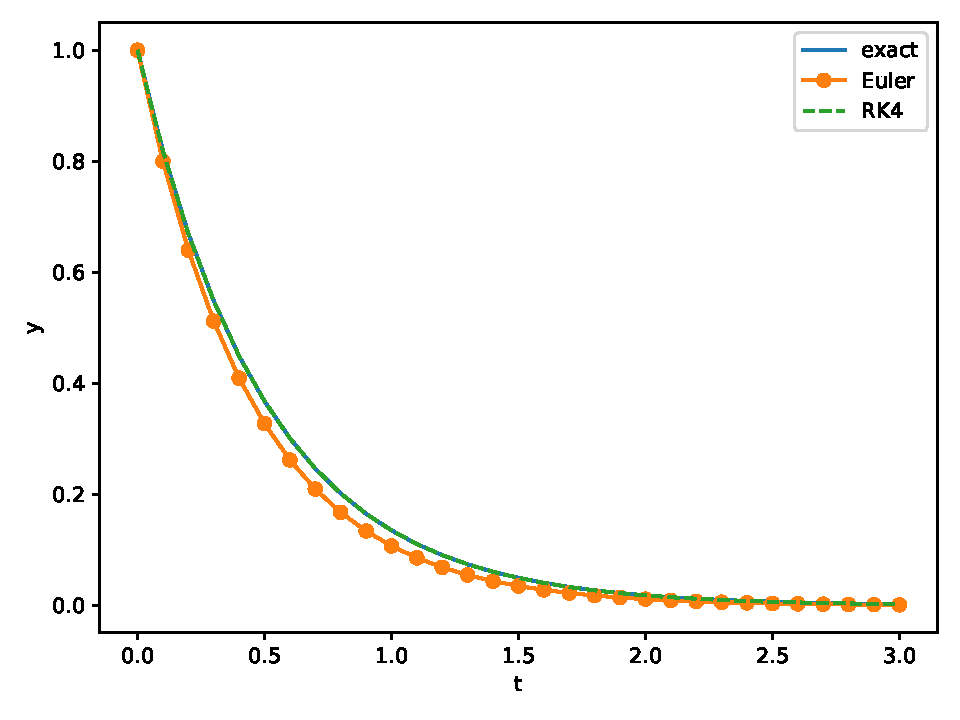
\includegraphics[width=0.47\textwidth]{generated/ch04/numerical_decay.pdf}\hfill
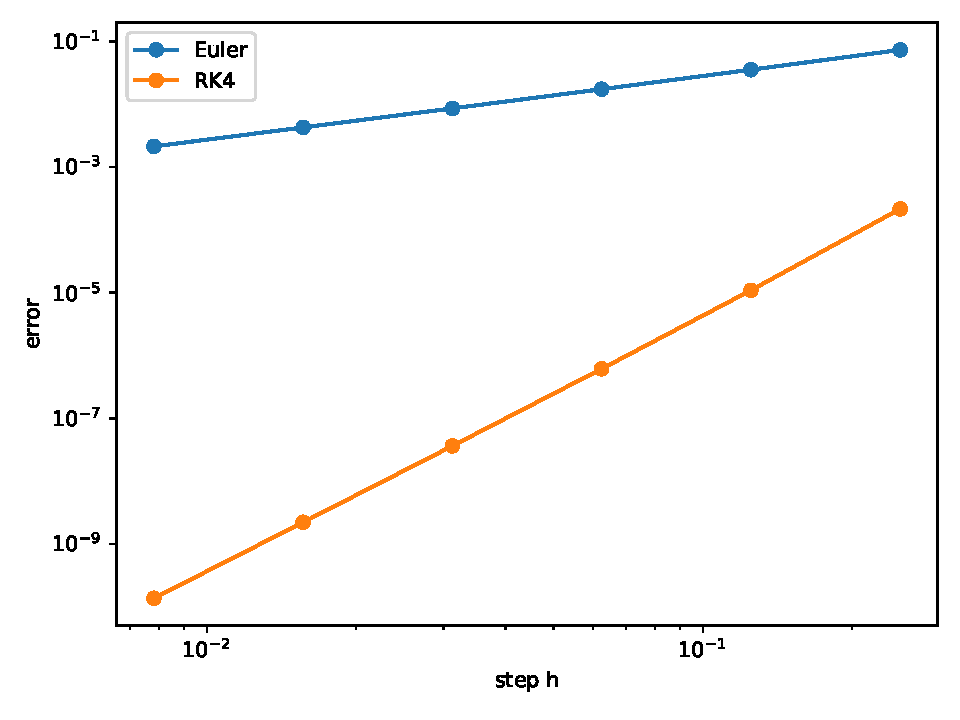
\includegraphics[width=0.47\textwidth]{generated/ch04/convergence.pdf}\par\medskip
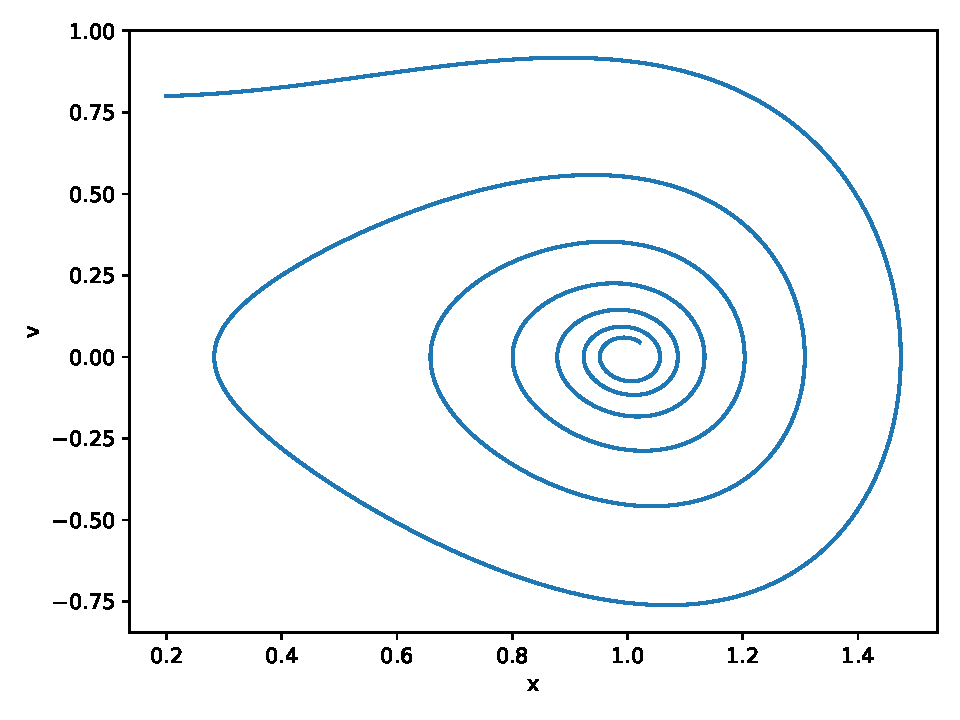
\includegraphics[width=0.47\textwidth]{generated/ch04/phase_portrait.pdf}\hfill
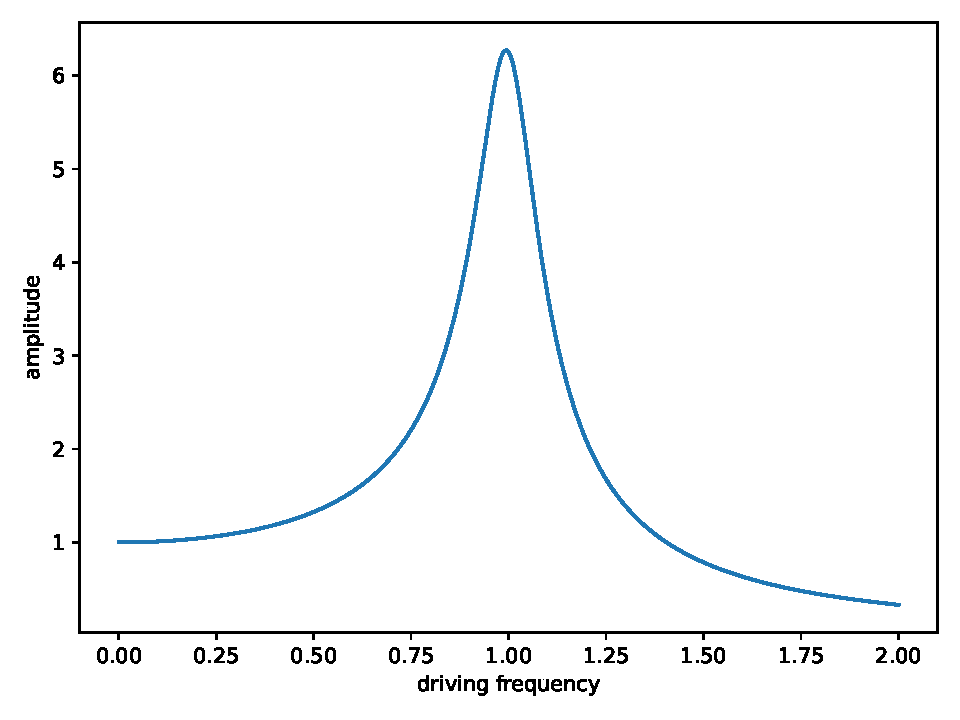
\includegraphics[width=0.47\textwidth]{generated/ch04/resonance_curve.pdf}
\end{minipage}
\end{bookfigure}
\subsection{Wolfram Language workflow}
The matching file \texttt{examples/wolfram/ch04/dynamical\_systems\_companion.wl} uses \texttt{DSolve}, \texttt{NDSolve}, and \texttt{ParametricPlot}.
\begin{warningbox}
Always test convergence under step refinement and compare against an analytic case. A smooth plot is not proof of numerical correctness.
\end{warningbox}

\section{Differential Equations Across Physics}
\label{sec:ch4-physics-applications}
Differential equations are the form in which local laws become predictions. The same patterns recur because inertia, storage, transport, feedback, and symmetry recur.
\subsection{Mechanics}
Newton's law $m\ddot{\mathbf r}=\mathbf F(\mathbf r,\dot{\mathbf r},t)$ is a second-order vector equation. Introducing velocity or momentum converts it into a first-order phase-space system. Conservative forces create energy surfaces; damping contracts trajectories; forcing creates resonance and can generate chaos.
\begin{physical}
The state-space language developed here leads directly to Lagrange's equations, Hamilton's canonical equations, normal modes, and perturbation theory.
\end{physical}
\subsection{Circuits}
Capacitance stores electric energy, inductance stores magnetic energy, and resistance dissipates it. RC circuits obey first-order relaxation equations, while RLC circuits obey the same second-order equation as a damped driven oscillator.
\subsection{Fields}
Separation of variables converts many field equations into families of ODEs. Wave equations produce oscillator equations for modes; diffusion produces exponential decay; radial symmetry reduces electrostatic, gravitational, and quantum problems to radial ODEs.
\subsection{Quantum evolution}
The time-dependent Schrödinger equation
\[i\hbar\frac{d}{dt}|\psi(t)\rangle=\hat H|\psi(t)\rangle\]
is a first-order linear equation in a complex vector space. For constant $\hat H$, an operator exponential generates unitary, norm-preserving evolution.
\subsection{Relativity and field theory}
Symmetry reduction and mode decomposition turn Maxwell, Klein--Gordon, Dirac, and Einstein equations into ODE systems. Cosmological expansion, geodesics, atomic radial functions, and renormalization-group flows all use the dynamical ideas introduced here.
\begin{keyidea}
Identify the state, write its local rate of change, locate equilibria or invariants, and determine how initial data propagate. The symbols change across physics, but the dynamical logic remains.
\end{keyidea}
\subsection{Looking ahead}
State space, generators, normal modes, and stability now form a bridge to classical mechanics, electromagnetism, quantum mechanics, and nonlinear field dynamics.

\section{Graded Exercise Bank}
\label{sec:ch4-exercises}

The following one hundred exercises form a cumulative assessment of Chapter~\ref{chap:04-ordinary-differential-equations}. They progress from solution fluency to modelling, qualitative dynamics, numerical analysis, and research-style computation. Unless otherwise stated, constants are real, physical parameters are positive, and all functions possess the regularity required by the indicated operations.

\subsection*{Tier I: Foundations (30 problems)}
\begin{enumerate}[label=\textbf{\arabic*.},leftmargin=*]
\item Classify the equation $y'+3y=0$ by order, linearity, and autonomy.
\item Verify that $y=Ce^{-2t}$ solves $y'+2y=0$.
\item Solve $y'=4y$ with $y(0)=3$.
\item Solve $y'=-ky$ with $y(0)=N_0$ and identify the characteristic time.
\item Find all equilibria of $y'=y(1-y)$.
\item Determine the sign of $y'$ for $y'=y(2-y)$ on the intervals separated by its equilibria.
\item Solve the separable equation $y'=t(1+y^2)$ with $y(0)=0$.
\item Solve $y'+y=t$ using an integrating factor.
\item Solve $y'-2y=e^{3t}$ with $y(0)=1$.
\item Find the half-life of a sample satisfying $N'=-\lambda N$.
\item Write Newton's cooling law as an initial-value problem for an object placed in a bath of constant temperature.
\item Solve the charging equation $RC\,q'+q=CV_0$ with $q(0)=0$.
\item Convert $x''+4x=0$ into a first-order system.
\item Find the characteristic roots of $x''+5x'+6x=0$.
\item Solve $x''+9x=0$ with $x(0)=A$ and $x'(0)=0$.
\item Compute the conserved energy of $x=A\cos(\omega t)$ for $m x''+kx=0$.
\item Classify the damping regime of $x''+4x'+4x=0$.
\item Find the general solution of $x''+2x'+5x=0$.
\item Find a particular solution of $x''+x=\cos 2t$.
\item State the resonance condition for an undamped driven oscillator.
\item Find the equilibrium points of $x'=x-y$, $y'=x+y$.
\item Write $\mathbf x'=A\mathbf x$ for the system $x'=2x+y$, $y'=x+2y$.
\item Find the eigenvalues of $A=\begin{pmatrix}2&1\\1&2\end{pmatrix}$.
\item Classify the origin for $\mathbf x'=\operatorname{diag}(-1,-3)\mathbf x$.
\item Classify the origin for $\mathbf x'=\operatorname{diag}(1,-1)\mathbf x$.
\item Sketch the phase portrait of $x'=y$, $y'=-x$.
\item Evaluate one Euler step for $y'=-y$, $y(0)=1$, with step $h=0.1$.
\item Evaluate two Euler steps for the same problem and compare with $e^{-0.2}$.
\item Explain the distinction between a direction field and a phase portrait.
\item Explain why an initial condition selects one trajectory from a solution family.
\end{enumerate}

\subsection*{Tier II: Intermediate synthesis (30 problems)}
\begin{enumerate}[label=\textbf{\arabic*.},leftmargin=*]
\item Solve the logistic initial-value problem $P'=rP(1-P/K)$, $P(0)=P_0$, and identify the carrying capacity.
\item Determine the stability of every equilibrium of $y'=y(y-1)(2-y)$.
\item Solve $y'+(2/t)y=t^2$ for $t>0$.
\item Solve the Bernoulli equation $y'+y=y^2$ by the substitution $u=1/y$.
\item Determine whether $(2xy+y^2)\,dx+(x^2+2xy)\,dy=0$ is exact and solve it.
\item Model a tank containing a dissolved substance when well-mixed fluid enters and leaves at equal rates.
\item Derive the terminal velocity for a falling body with linear drag $m v'=mg-bv$.
\item Solve $m v'=F_0-bv$ with $v(0)=0$ and interpret the relaxation time.
\item Find the current in an RL circuit satisfying $L I'+RI=V_0$, $I(0)=0$.
\item Solve the discharging RC equation and find the time at which the voltage falls to ten percent of its initial value.
\item Solve $x''-x'-6x=0$ with $x(0)=0$, $x'(0)=1$.
\item For $m x''+b x'+kx=0$, derive the critical-damping condition.
\item Find the amplitude and phase lag of the steady response to $m x''+b x'+kx=F_0\cos\Omega t$.
\item Show that the average power absorbed by a driven oscillator is maximized near resonance.
\item Derive the small-angle pendulum equation from $\theta''+(g/\ell)\sin\theta=0$.
\item Estimate the relative period error caused by the small-angle approximation at a moderate initial angle.
\item Diagonalize $A=\begin{pmatrix}0&1\\-2&-3\end{pmatrix}$ and solve $\mathbf x'=A\mathbf x$.
\item Find the matrix exponential of a planar rotation generator $A=\begin{pmatrix}0&-\omega\\omega&0\end{pmatrix}$.
\item Derive the normal-mode frequencies of two identical masses coupled by three identical springs.
\item Show that the symmetric and antisymmetric normal modes evolve independently.
\item Classify a linear planar system from its trace and determinant.
\item Linearize $x'=x-x^3-y$, $y'=x-y$ at each equilibrium.
\item Use a quadratic Lyapunov function to establish stability of $x'=-ax$, $y'=-by$ for $a,b>0$.
\item Analyze the bifurcation of $x'=\mu x-x^3$ as $\mu$ passes through zero.
\item Compare Euler and midpoint methods on $y'=-2y$ over a fixed interval.
\item Derive the local truncation error of Euler's method by Taylor expansion.
\item Apply one RK4 step to $y'=t-y$, $y(0)=1$.
\item Explain absolute stability for the test equation $y'=\lambda y$.
\item Determine the Euler stability restriction when $\lambda<0$ is real.
\item Construct a numerical phase portrait for the damped pendulum and identify its attractor.
\end{enumerate}

\subsection*{Tier III: Advanced analysis (20 problems)}
\begin{enumerate}[label=\textbf{\arabic*.},leftmargin=*]
\item Prove uniqueness for $y'=f(t,y)$ under a local Lipschitz condition by estimating the difference of two solutions.
\item Give an example in which an initial-value problem has more than one solution because the Lipschitz condition fails.
\item Derive the variation-of-constants formula for $\mathbf x'=A\mathbf x+\mathbf f(t)$.
\item Prove that $e^{At}$ satisfies the semigroup property for a constant matrix $A$.
\item Derive Abel's identity for the Wronskian of a second-order linear equation.
\item Use the Wronskian to test linear independence of two oscillator solutions.
\item Construct the Green function for a forced oscillator with specified homogeneous initial conditions.
\item Show that damping makes the mechanical energy nonincreasing for $m x''+b x'+V'(x)=0$.
\item Analyze the nonlinear pendulum in phase space and identify separatrices.
\item Derive the energy-dependent period integral for the nonlinear pendulum.
\item Apply the Hartman--Grobman idea informally to a hyperbolic equilibrium and state its limitation.
\item Classify all phase portraits of a real $2	imes2$ linear system, including repeated and complex eigenvalues.
\item Show that a nontrivial periodic orbit cannot occur in a one-dimensional autonomous ODE.
\item Use the Bendixson--Dulac criterion to exclude periodic orbits in a specified planar model.
\item Nondimensionalize the driven damped oscillator and identify its independent dimensionless parameters.
\item Derive the modified equation associated with Euler's method through second order.
\item Prove the fourth-order global accuracy of RK4 under suitable smoothness assumptions at an outline level.
\item Explain stiffness using a two-timescale linear system and compare explicit and implicit Euler stability.
\item Derive Crank--Nicolson evolution for a linear system and discuss norm preservation for skew-Hermitian generators.
\item Show how separation of variables converts a linear PDE mode into an ODE eigenvalue problem.
\end{enumerate}

\subsection*{Tier IV: Challenge and computational investigations (20 problems)}
\begin{enumerate}[label=\textbf{\arabic*.},leftmargin=*]
\item Implement Euler, midpoint, and RK4 methods without using a library ODE solver; compare error versus step size on a problem with known solution.
\item Implement adaptive step-size control using step doubling and test it near a rapidly varying transient.
\item Compute and plot the resonance curve of an RLC circuit for several damping values.
\item Numerically locate the separatrix of the nonlinear pendulum and compare it with the analytic energy condition.
\item Construct a bifurcation diagram for $x'=\mu x-x^3$ and annotate stable and unstable branches.
\item Explore a saddle-node bifurcation numerically for $x'=\mu-x^2$.
\item Simulate the Lotka--Volterra model, derive its nontrivial equilibrium, and compare linearized and nonlinear trajectories.
\item Add logistic limitation to a predator--prey model and investigate whether a stable cycle persists.
\item Integrate the Duffing oscillator for several forcing amplitudes and compare phase portraits and Poincar'e sections.
\item Simulate the Lorenz equations and estimate sensitivity to initial conditions from two nearby trajectories.
\item Estimate the largest Lyapunov exponent of a chosen nonlinear system.
\item Construct a symplectic Euler integrator for the harmonic oscillator and compare long-time energy drift with standard Euler.
\item Implement velocity Verlet for a one-dimensional potential and test time reversibility.
\item Solve a two-mass coupled oscillator both by direct integration and by normal-mode decomposition.
\item Build a numerical propagator for a two-level quantum system and test norm conservation.
\item Compare explicit Euler, implicit Euler, and trapezoidal evolution on a stiff decay system.
\item Infer parameters of an exponential-decay model from synthetic noisy data and quantify uncertainty.
\item Fit a damped sinusoid to simulated data and discuss parameter correlations.
\item Create an interactive direction-field and solution-curve viewer for a user-entered first-order ODE.
\item Write a short modelling report that begins from a physical assumption, derives an ODE, nondimensionalizes it, solves or simulates it, and evaluates the model's limitations.
\end{enumerate}

\subsection*{Selected guidance}
\begin{description}[leftmargin=2.6cm,style=nextline]
\item[Foundation 7.] Separate variables and integrate: $\arctan y=t^2/2+C$; then impose the initial condition.
\item[Foundation 17.] The repeated characteristic root is $r=-2$; remember the second independent solution $t e^{-2t}$.
\item[Intermediate 13.] Substitute $x_p=a\cos\Omega t+b\sin\Omega t$, or use complex amplitudes, and separate magnitude from phase.
\item[Intermediate 21.] For $A=\begin{psmallmatrix}a&b\\c&d\end{psmallmatrix}$, use $\tau=a+d$ and $\Delta=ad-bc$, then examine $\tau^2-4\Delta$.
\item[Intermediate 29.] Euler is stable for $|1+h\lambda|<1$; solve this inequality for a negative real $\lambda$.
\item[Advanced 8.] Differentiate $E=\tfrac12m\dot x^2+V(x)$ and use the equation of motion to obtain $\dot E=-b\dot x^2$.
\item[Advanced 13.] Uniqueness prevents a trajectory from returning to the same state with a different derivative in one dimension.
\item[Challenge 12.] Track both phase-space geometry and the numerical energy error over many periods; short-time agreement alone is not sufficient.
\item[Challenge 15.] Use a unitary exponential or a norm-preserving time integrator as the reference method.
\item[Challenge 20.] State assumptions, dimensions, parameters, initial data, validation criteria, and failure modes explicitly.
\end{description}

\section{Repository Integration and Chapter Dependencies}
\label{sec:ch4-integration}

The vocabulary of this chapter is now part of the book-wide glossary and notation system. In particular, \gls{ordinarydifferentialequation}, \gls{initialvalueproblem}, \gls{directionfield}, \gls{phasespace}, \gls{equilibrium}, \gls{stability}, \gls{bifurcation}, and \gls{stiffness} are used consistently in later chapters. The canonical state-space convention is
\[
\dot{\mathbf x}=\mathbf f(t,\mathbf x),
\qquad
\mathbf x(t_0)=\mathbf x_0,
\]
while autonomous systems omit the explicit time argument.

\begin{physicalbox}[Dependency map: from laws of change to physics]
\[
\begin{array}{c}
\text{initial-value problem}\longrightarrow\text{trajectory}\longrightarrow\text{phase flow}\\[2mm]
\downarrow\hspace{30mm}\downarrow\hspace{30mm}\downarrow\\[-1mm]
\text{Newtonian motion}\qquad\text{circuit dynamics}\qquad\text{quantum evolution}
\end{array}
\]
Chapter~\ref{ch:mathematical-language-of-physics} supplies vectors and eigenmodes; Chapter~\ref{ch:differential-calculus} supplies linearization and Jacobians; Chapter~\ref{ch:vector-calculus} supplies spatial field operators. This chapter combines them into evolution laws. Later mechanics chapters use second-order equations and phase space, electromagnetism uses coupled first-order field evolution, and quantum mechanics uses linear state evolution generated by a Hamiltonian.
\end{physicalbox}

\index{ordinary differential equation}
\index{initial-value problem}
\index{direction field}
\index{phase space}
\index{equilibrium point}
\index{stability}
\index{bifurcation}
\index{stiffness}
\index{Runge--Kutta method}
\index{harmonic oscillator}

\section{Summary and Looking Ahead}
\label{sec:ch4-summary}

An ordinary differential equation converts a local law of change into a trajectory. First-order equations describe relaxation, transport between compartments, growth, and circuit response. Second-order equations describe inertia, oscillation, damping, and resonance. Systems of equations expose eigenmodes and coupled motion, while phase space replaces a single graph by a geometric flow of possible states. Equilibria, linearization, Lyapunov functions, and bifurcations distinguish persistence from instability and reveal how qualitative behavior changes with parameters.

Analytical formulas remain indispensable, but numerical integration is part of the mathematical theory rather than an afterthought. Step size, consistency, stability, stiffness, invariants, and error control determine whether a computed trajectory represents the differential equation or merely the algorithm.

The central pattern is
\[
\boxed{\begin{gathered}
\text{physical assumption}\longrightarrow\text{differential equation}
\longrightarrow\text{initial data}\\
\longrightarrow\text{evolution}\longrightarrow\text{interpretation}
\end{gathered}}
\]
This pattern will recur throughout the book. Newton's laws become dynamical systems; Maxwell's equations propagate fields; the Schr\"odinger equation evolves quantum states; and relativistic field equations determine the geometry and matter content of spacetime. The next chapter extends the mathematical foundation needed to analyze these theories with greater structural precision.

